\documentclass[journal=jcisd8,manuscript=article,layout=traditional]{achemso}
\setkeys{acs}{articletitle=true,etalmode=truncate,maxauthors=10}

\usepackage{float}
\usepackage{enumitem}
\usepackage{amsmath}
\usepackage{booktabs}
\usepackage{graphicx}
\usepackage{url}
\usepackage{stfloats}
\usepackage{tabularx}
\usepackage{adjustbox}
\usepackage{xcolor}
\usepackage[T1]{fontenc}
\usepackage{lmodern}
\usepackage[utf8]{inputenc}
\usepackage{microtype}
\usepackage{inconsolata}

% TBD placeholders are filled from results/paper_values.json by scripts/06_fill_paper.py.
\newif\ifshowTBDkeys
\showTBDkeysfalse
\newcommand{\TBD}[1]{\textcolor{red}{[\textbf{TBD}: \nolinkurl{#1}]}}
\newcommand{\TBDtext}[2]{\textcolor{red}{[\textbf{TBD} \nolinkurl{#1}: \emph{#2}]}}
\newcommand{\TBDcell}[1]{\ifshowTBDkeys\textcolor{red}{\scriptsize\texttt{\detokenize{#1}}}\else\textcolor{red}{TBD}\fi}
\newcommand{\FIGTBD}[2]{\fbox{\parbox[c][4.5cm][c]{0.9\linewidth}{\centering\textcolor{red}{\textbf{Figure placeholder}}\\[2pt]\texttt{\detokenize{#1}}\\[2pt]\small #2}}}

\emergencystretch=3em
\renewcommand*\tocentryname{For Table of Contents Only}

\title{Publication-aware prediction of battery material properties from literature-extracted data}
\author{Sunraj Patel}
\email{sunrajpatelcph@gmail.com}
\affiliation{Department of Materials Science and Engineering, Indian Institute of Technology Kanpur, Kanpur 208016, India}

\begin{document}

\begin{tocentry}
\centering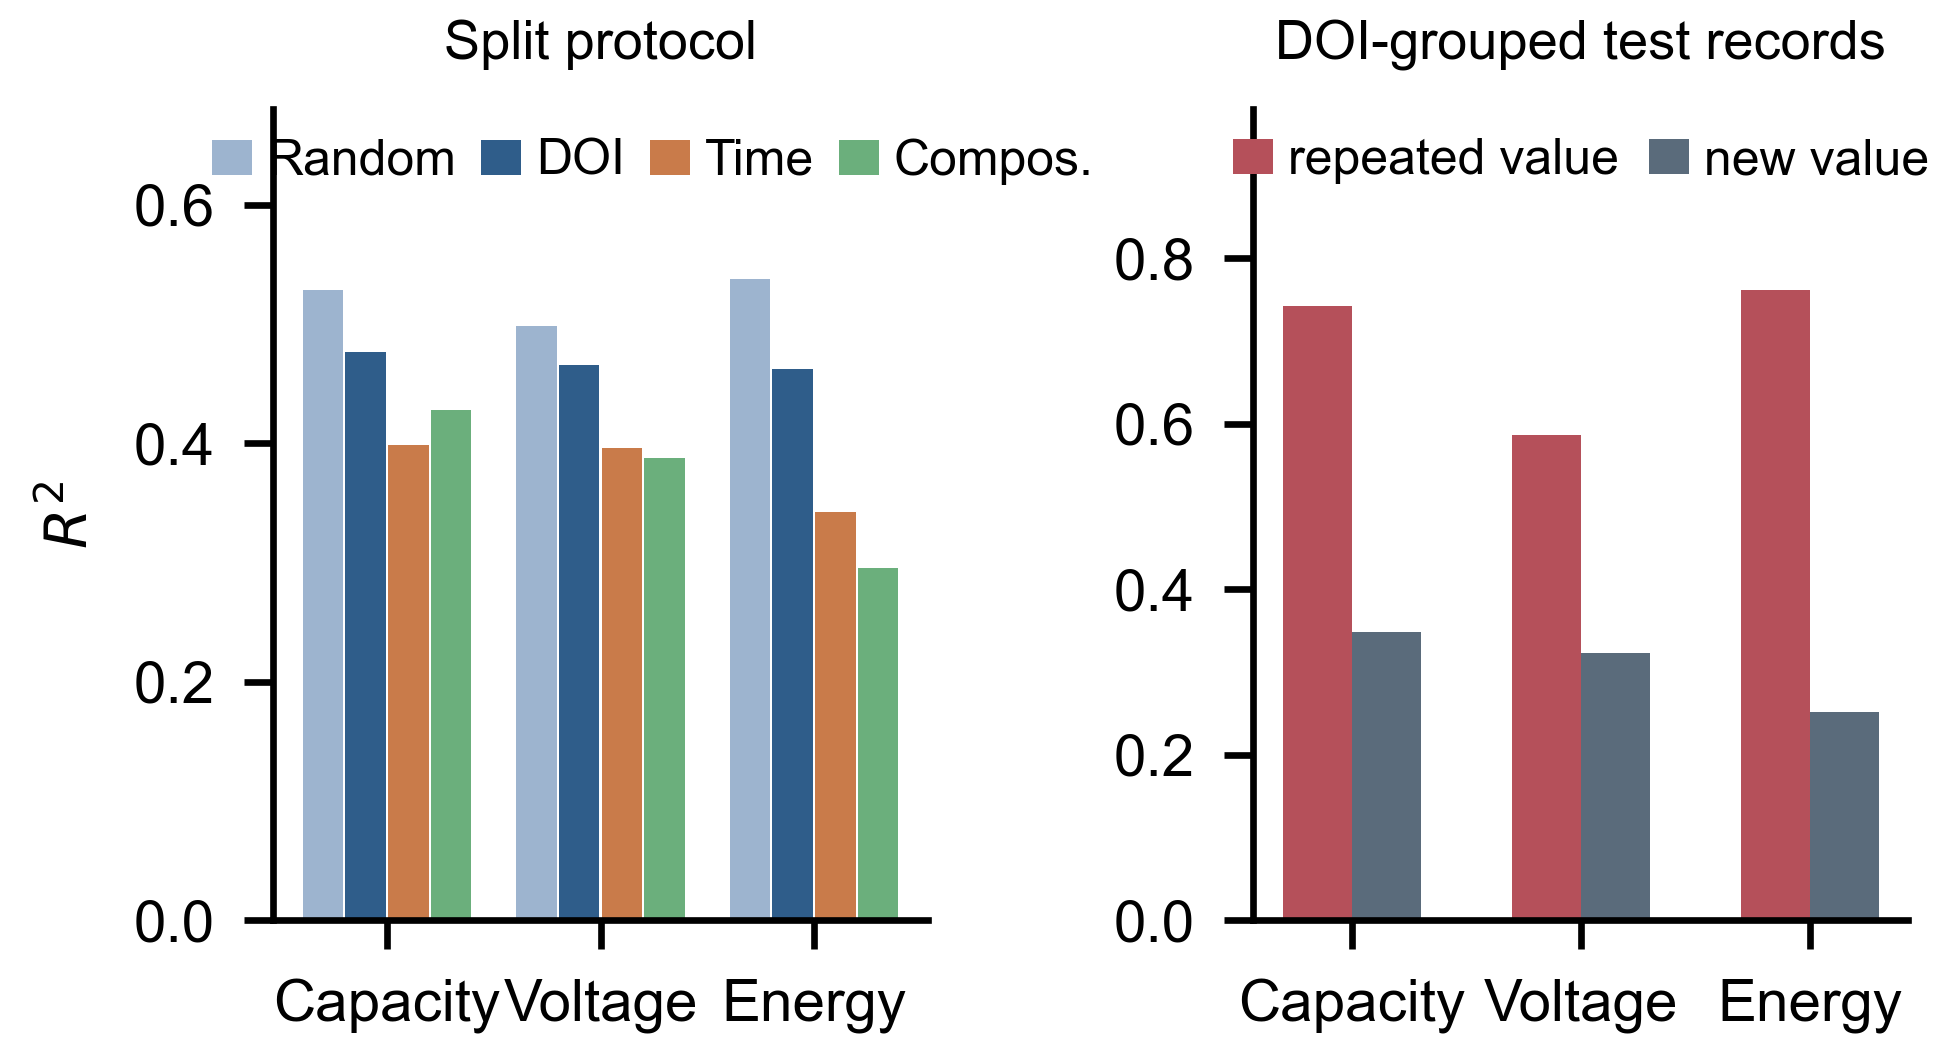
\includegraphics[width=3.25in]{figures/toc.png}
\end{tocentry}

\begin{abstract}
Text-mined databases are attractive training sources for property-prediction models, but their records are clustered by publication; we trained CatBoost--XGBoost ensembles for capacity, voltage, $\log_{10}$ conductivity, Coulombic efficiency and energy on 285,243 records of the auto-generated Huang--Cole battery database and evaluated identical models under record-level, publication-grouped (DOI), temporal and composition-grouped splits. Although 30--84\% of target variance lies between publications, DOI grouping lowered $R^2$ only modestly (capacity 0.529 $\pm$ 0.009 to 0.477 $\pm$ 0.015 with the conservative main feature set, and 0.574 $\pm$ 0.009 to 0.523 $\pm$ 0.014 with title keywords describing the cell chemistry), because composition descriptors carry little recoverable publication identity. A leakage route that survives DOI grouping is values recurring across the literature: 16--46\% of DOI-grouped test records repeat a (material, value) pair reported by another publication in training and are predicted far better (capacity $R^2$ 0.74 versus 0.35), while conductivity and Coulombic efficiency are not usefully predictable ($R^2$ 0.10 and 0.05 on values without a precedent). Publication-grouped evaluation is therefore necessary but not sufficient, and we recommend composition-grouped or temporal splits, a repeated-value breakdown and a bibliographic-fingerprint test, implemented in an auditable pipeline that also re-runs the two previous regression pipelines on the same database.
\end{abstract}

\section{Introduction}
\label{sec:intro}

The performance of a rechargeable battery is bounded by the properties of its electrode and electrolyte materials (Figure~\ref{fig:cell}). Specific capacity and the average electrode potential together set the specific energy of a cell, the conductivity of the electrolyte limits rate capability, and the Coulombic efficiency measures the charge lost to side reactions in each cycle. Thousands of papers report these quantities every year, each for one or a few materials and under conditions, such as current density and cycle number, that the authors choose.

\begin{figure}[htbp]
    \centering
    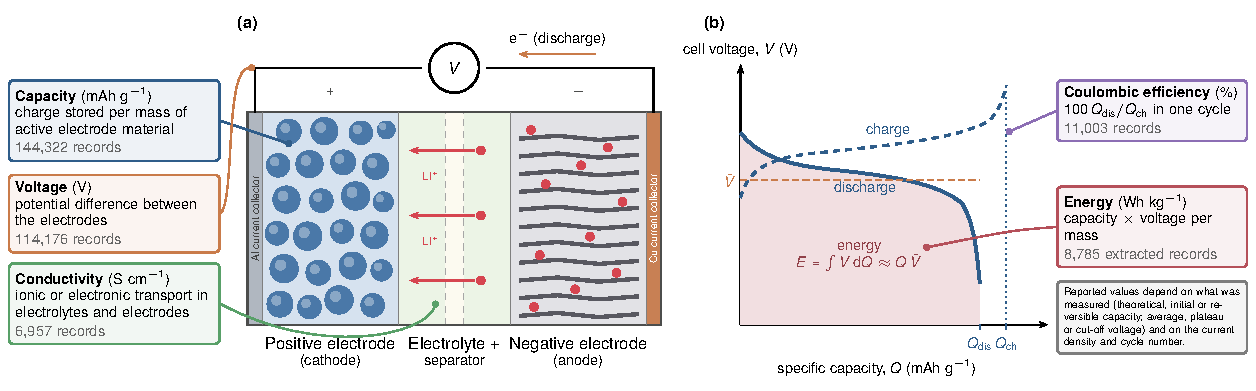
\includegraphics[width=\linewidth]{figures/battery_cell.pdf}
    \caption{\textbf{The five properties in the Huang--Cole database.} (a) Schematic of a lithium-ion cell during discharge, with the quantities reported for electrode and electrolyte materials. (b) Idealised galvanostatic charge (dashed) and discharge (solid) curves: specific capacity $Q$, average voltage $\bar V$, energy as the area under the discharge curve, and Coulombic efficiency as the ratio of discharge to charge capacity. Record counts are those of the cleaned modelling sets.}
    \label{fig:cell}
\end{figure}

Text-mining tools such as ChemDataExtractor \cite{swain2016chemdataextractor,mavracic2021chemdataextractor2} turn this literature into structured data. Huang and Cole applied a battery-specific version to 229,061 papers and obtained 292,313 records of capacity, voltage, conductivity, Coulombic efficiency and energy, with an estimated precision of 80\% \cite{huang2020database,huang2020figshare}. Earlier ML work on battery materials was limited to a few hundred manually digitised cathode records \cite{kauwe2019battery,ghadbeigi2015performance}, and cell-level models are trained on cycling data from a single controlled campaign \cite{severson2019cyclelife}; a database of this size is an obvious alternative training source. Two groups have trained regressors on it, both evaluated with random record-level splits \cite{zhuang2024property,jablonka2026clever}.

Literature-derived records are, however, clustered by publication. One paper may report capacities at several current densities and cycles, for a parent material and its doped or coated variants, all measured in one laboratory; Huang and Cole flag about 40\% of the records as members of such within-paper series \cite{huang2020database}. Under a random split most test records have siblings from the same paper in training, and a model can score well by recognising the paper rather than by learning how a material determines its properties. Grouped, cluster-based and time-split validation are the established remedies \cite{roberts2017crossvalidation,meredig2018cluster,witman2025matfold,sheridan2013timesplit,kapoor2023leakage}, and Jablonka recently showed that composition descriptors can predict the authors, journal and year of a record, so that models may succeed for bibliographic rather than chemical reasons \cite{jablonka2026clever}. Grouping by source publication, the natural unit of dependence in a text-mined database, has not been reported for this database.

Here we ask how much this structure changes the evaluation of models trained on the Huang--Cole database (Figure~\ref{fig:workflow}). The answer is not the one a simple leakage argument predicts: the records are strongly clustered by publication, yet record-level and DOI-grouped estimates differ only modestly. We trace this to two mechanisms. The available features identify publications poorly, and many reported values recur across publications, so that a DOI-grouped split still lets a model recall them. Our contributions are:

\begin{enumerate}[label=(\roman*),itemsep=1pt]
    \item an evaluation of five properties under record-level random, DOI-grouped, temporal and composition-grouped splits with the same model and features, together with the share of each target's variance that lies between publications;
    \item an analysis of leakage channels beyond publication identity: recoverable bibliographic information, values that recur across publications, and theoretical capacities;
    \item an auditable feature construction, with every excluded column and the treatment of the database's warning flags documented, and noise, paper-level-feature, identity and within-paper-series controls;
    \item a comparison with the two previous regression pipelines on the same database, re-run on identical partitions.
\end{enumerate}

\begin{figure}[htbp]
    \centering
    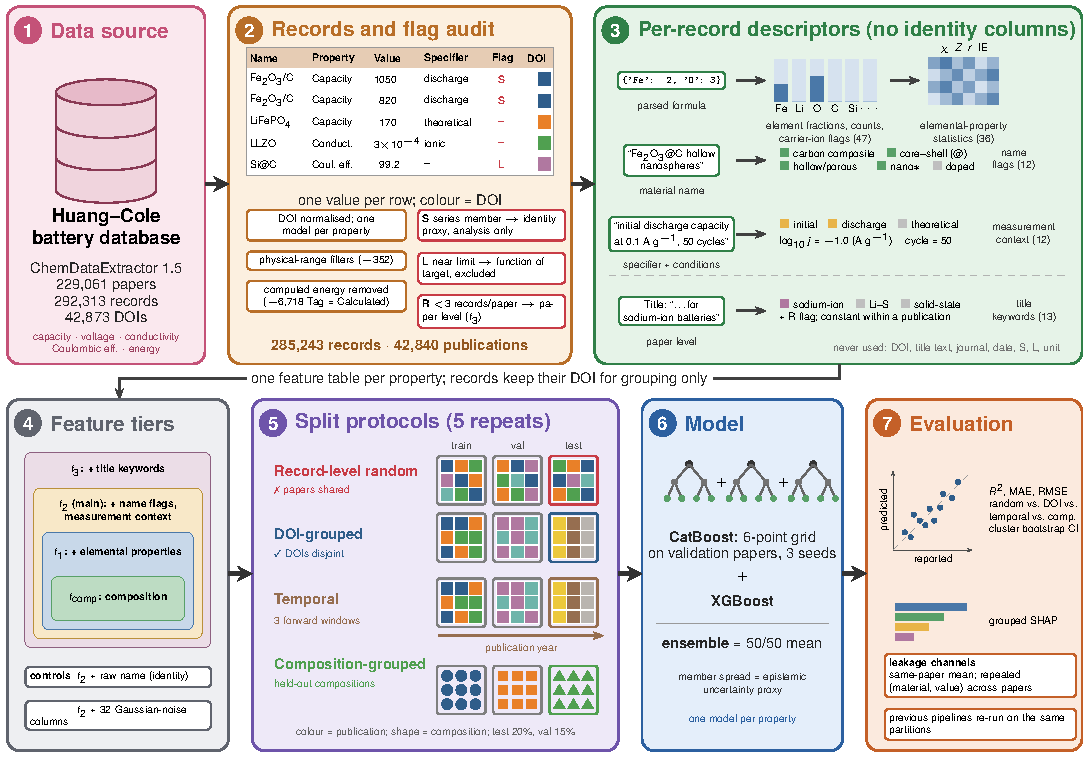
\includegraphics[width=\linewidth]{figures/workflow.pdf}
    \caption{\textbf{Workflow for publication-aware prediction of battery material properties.} (1) The un-merged Huang--Cole records. (2) Records are kept in long format with their DOI, cleaned with physical-range filters, and the database's warning flags are audited: S marks within-paper series and acts as a publication-identity proxy (analysis only), L is a function of the target (excluded) and R is paper-level (title tier only). (3) Descriptors are computed per record from the parsed formula, the material name, the property specifier and conditions, and (separately) the paper title; identity and target-derived columns are never used. (4) Nested feature tiers and controls. (5) Each target is evaluated under record-level random, DOI-grouped, temporal and composition-grouped splits. (6) A CatBoost--XGBoost ensemble is trained per property. (7) Evaluation, grouped SHAP attribution, ensemble-spread uncertainty, leakage-channel analyses and re-runs of previous pipelines.}
    \label{fig:workflow}
\end{figure}

% ---------------- METHODS ----------------
\section{Methods}

\subsection{Data Preparation}

\subsubsection{Dataset Description}
\label{sec:data}

We used the un-merged file \texttt{battery.csv} from the Huang--Cole release \cite{huang2020figshare}, which contains one row per extracted record: 292,313 records from 42,873 DOIs (Table~\ref{tab:dataset}). The release also contains a merged file in which identical (compound, property, value) triples from different papers are collapsed into one row with a record count. Merging removes the link between a record and its publication, which is required for grouped evaluation, so the merged file was not used.

The data are in long format. Each record carries one value of one property (\texttt{Property}, \texttt{Value}, normalised \texttt{Unit}, and the text as written in \texttt{Raw\_value} and \texttt{Raw\_unit}), the compound name as it appears in the text (\texttt{Name}), its parsed composition (\texttt{Extracted\_name}, a list of element--stoichiometry dictionaries), the property specifier recognised by the parser (\texttt{Specifier}), and publication metadata (\texttt{DOI}, \texttt{Title}, \texttt{Journal}, \texttt{Date}). Three further fields are sparse: \texttt{Info} stores the current density and cycle number found next to a capacity value; \texttt{Type} records whether the material was identified as a cathode, anode or electrolyte and is populated for about 3\% of records; and \texttt{Correctness} holds the manual evaluation labels for the validation sample of about 500 records \cite{huang2020database}. The \texttt{Tag} field marks 6,718 energy records as \emph{Calculated}: these were derived by Huang and Cole from capacity and voltage records of the same material rather than extracted from text. The \texttt{Warning} field is described in Section~\ref{sec:warnings}.

Two properties of this structure matter for what follows. First, there is no record that describes a cell or an experiment as a whole: the capacity and voltage of the same material in the same paper are separate records, and they cannot in general be joined because the database does not identify which values were measured together. Each property is therefore modelled separately. Second, the predictors available for a record are limited to what can be read from the compound name, its composition, the specifier and a few conditions. Electrode formulation, loading, electrolyte, counter electrode, voltage window and temperature, which strongly influence measured capacity and Coulombic efficiency, are not recorded.

\begin{table}[htbp]
    \centering\small
    \caption{\textbf{Records in the Huang--Cole database and in the modelling sets.} Raw counts are from \texttt{battery.csv}; publications are unique DOIs after normalisation. Cleaned counts are after the filters in Section~\ref{sec:cleaning}.}
    \label{tab:dataset}
    \begin{adjustbox}{max width=\textwidth}
    \begin{tabular}{@{}lrrrr@{}}
        \toprule
        Property & Raw records & Raw publications & Modelling records & Modelling publications \\
        \midrule
        Capacity               & 144,359 & 22,836 & 144,322 & 22,833 \\
        Voltage                & 114,240 & 32,754 & 114,176 & 32,747 \\
        Energy                 &  15,543 & 3,129 & 8,785 & 3,113 \\
        Coulombic efficiency   &  11,003 & 5,861 & 11,003 & 5,861 \\
        Conductivity           &   7,168 & 3,482 & 6,957 & 3,351 \\
        \midrule
        Total                  & 292,313 & 42,873 & 285,243 & 42,840 \\
        \midrule
        \multicolumn{5}{@{}l}{\textbf{Flags in the raw file}} \\
        \multicolumn{3}{@{}l}{\texttt{Tag} = Calculated (energy only)} & \multicolumn{2}{r}{6,718} \\
        \multicolumn{3}{@{}l}{\texttt{Warning} = S / L / LS / R / RL} & \multicolumn{2}{r}{99,671 / 33,858 / 17,732 / 7,999 / 3,338} \\
        \multicolumn{3}{@{}l}{\texttt{Type} populated} & \multicolumn{2}{r}{$\approx$3\%} \\
        \multicolumn{3}{@{}l}{\texttt{Correctness} populated (manual sample)} & \multicolumn{2}{r}{$\approx$500} \\
        \bottomrule
    \end{tabular}
    \end{adjustbox}
\end{table}

\subsubsection{Targets}
\label{sec:targets}

One regression model was trained per property (Table~\ref{tab:targets}). Conductivity was modelled as $\log_{10}(\sigma / \mathrm{S\,cm^{-1}})$ because reported values span many orders of magnitude and the physically meaningful error is multiplicative; its MAE and RMSE are therefore in decades. All other targets were modelled in their normalised units. A small fraction of capacity records carry the unit Ah~kg$^{-1}$, which is numerically identical to mAh~g$^{-1}$, and were kept.

The five targets are not equally well defined. ``Capacity'' pools theoretical, initial, reversible, charge and discharge capacities at different current densities and cycle numbers; ``voltage'' pools average, plateau, open-circuit and cut-off voltages; ``conductivity'' pools ionic and electronic conductivities of electrolytes and electrodes. The specifier and the parsed conditions are given to the model as features (Section~\ref{sec:features}), but a large part of the target variance is due to what was measured rather than to the material, and this sets a ceiling on achievable accuracy.

\subsection{Literature Corpus and Automated Extraction}

\subsubsection{Huang--Cole corpus}

The corpus is the output of the battery-specific ChemDataExtractor pipeline built by Huang and Cole \cite{huang2020database,huang2020figshare}, which was applied to 229,061 papers. The database stores each extracted value as a separate record, together with the compound name, its parsed elemental composition, the property specifier (for example ``discharge capacity'' or ``theoretical capacity''), additional conditions for capacity (current and cycle), the DOI, title, journal and publication date. This study does not perform any extraction of its own, and no large-language-model extraction was used: all information about the literature comes from the released records, and the released Correctness labels and Warning flags are the only quality information available. Later extraction approaches \cite{huang2022batterybert,xu2024atomworkbattery,dagdelen2024structured} are discussed as related work only.

\subsubsection{Warning flags}
\label{sec:warnings}

Huang and Cole attach three warning flags to records \cite{huang2020database}, and each needs a decision.

\textbf{S (series).} A record is flagged S when values occur more than three times with the same compound name, property and DOI, i.e.\ when it belongs to a data series such as capacity versus cycle number or versus current density. In the raw file 99,671 records carry S alone and 17,732 carry L and S together. The S flag is a direct function of how many sibling records a publication contributes for the same material, so it encodes publication identity rather than material properties. It is not used as a predictor. Because series members are strongly correlated with one another, they are also the records through which a random split leaks most information. We therefore report, as a sensitivity analysis, all results with the S records removed (Section~\ref{sec:series}).

\textbf{L (near limit).} A record is flagged L when its value lies in a ``near limit'' region defined by fixed value ranges (for example 0--20 and 3,000--5,000~mAh~g$^{-1}$ for capacity, 0--1 and 5--8~V for voltage, 0--20\% for Coulombic efficiency) \cite{huang2020database}. L is therefore a deterministic function of the target value. Using it as a feature would tell the model that the target lies in one of two tails, which is target leakage. L is not used as a predictor; L-flagged records are retained if they pass our own range filter, and their share of the error is reported separately (capacity: 2\% of test records, 5\% of absolute error; voltage: 41\% of test records, 42\% of absolute error).

\textbf{R (relevance).} A record is flagged R when fewer than three records were extracted from its article, a heuristic for papers that are not primarily about battery materials \cite{huang2020database}. R is constant within a publication and does not depend on the target. Because it is a paper-level constant, it is admitted only in the paper-level block (\texttt{lit\_warn\_R}, tier \texttt{t3}) together with the title keywords, and is assessed in the same way (Section~\ref{sec:controls}).

\subsubsection{Correctness sample}
\label{sec:quality}

Huang and Cole evaluated the database on about 500 records drawn by random shuffling and supplemented by hand with additional records for the rarer properties \cite{huang2020database}. Precision was 83.3\% for capacity, 79.0\% for voltage, 76.0\% for conductivity, 77.6\% for Coulombic efficiency and 75.5\% for energy (80.0\% overall); recall, estimated on 51 papers, was 59.1\% overall. A record was counted as correct when the compound name, value, property and unit all matched the source text. Errors were classified as incomplete composites (F1, e.g.\ only ``rGO'' extracted from ``N-ZnSe@rGO''), incorrect names (F2), incorrect matches between a value and a compound or property (F3, the most common type), and interdependency errors (F4). The resulting labels are stored in the \texttt{Correctness} column of the release, which we use only for analysis and never as a feature.

\subsection{Feature Engineering}
\label{sec:features}

Every feature is computed from the fields of a single record. Features are organised in blocks, identified by a column prefix, that define both the feature tiers and the groups used for SHAP aggregation (Table~\ref{tab:predictors}).

\subsubsection{Composition and Elemental-Property Descriptors}

\textbf{Composition} (\texttt{comp\_}). Atomic fractions of a predeclared list of elements, comprising every element present in at least 0.5\% of cleaned records; the list was computed once from the full corpus before any split and frozen. The block also contains the number of elements, the number of components in \texttt{Extracted\_name} (composites are parsed as several components), and indicator flags for the common carrier ions (Li, Na, K, Mg, Zn, Al).

\textbf{Elemental properties} (\texttt{mat\_}). Stoichiometry-weighted mean, minimum, maximum and range of tabulated elemental properties (atomic number, atomic mass, Pauling electronegativity, atomic radius, period, group, Mendeleev number, first ionisation energy and a common-oxidation-state proxy), computed with pymatgen \cite{ong2013pymatgen} in the manner of Magpie descriptors \cite{ward2016magpie}. Because it is computed from composition, this block adds no information that is not already implicit in the composition block, but it presents that information in a form tree models can split on.

\subsubsection{Name, Measurement and Paper-Level Features}

\textbf{Material name} (\texttt{txt\_}). Regular-expression flags on \texttt{Name} for words a materials scientist would read as architecture or morphology: carbon, graphene, CNT and rGO composites; core--shell (``@''); slash composites; doping; nano-prefixes; hollow and porous structures; films; and the words anode, cathode and electrode.

\textbf{Measurement context} (\texttt{meas\_}). Keyword flags on \texttt{Specifier} (theoretical, reversible, discharge, charge, specific, electronic/electrical, potential; the release contains only 54 distinct specifier strings, so further candidate keywords such as initial, areal, volumetric, open-circuit or cut-off never occur and were not used) and a flag for a missing specifier; current density parsed from \texttt{Info}, normalised to A~g$^{-1}$ where the unit allows and $\log_{10}$-transformed, with C-rate and cycle number where present and a missingness indicator for each; and \texttt{Type} as a categorical variable (cathode, anode, electrolyte, unknown).

\textbf{Paper-level title keywords} (\texttt{lit\_}). Flags for battery chemistry and topic words in \texttt{Title} (lithium-ion, sodium-ion, potassium, Li--S, Li--O$_2$/air, zinc, magnesium, supercapacitor, solid-state, electrolyte, anode, cathode), together with the R flag as \texttt{lit\_warn\_R}. In the released file titles are stored upper-case with spaces and stop words removed (e.g.\ \texttt{...ANODESFORLITHIUMIONBATTERIES}), so the patterns match substrings. These features are constant within a publication, which is exactly the property that makes paper-level features suspect under record-level splitting.

\textbf{Material identity} (\texttt{id\_name}). The lower-cased, whitespace-normalised \texttt{Name} string as a CatBoost categorical variable. Used only in the identity-admission control.

\textbf{Noise} (\texttt{noise\_}). 32 independent standard-normal columns, used only in the negative control.

Preprocessing was fitted on each training partition: features missing in more than 80\% of training records were dropped, except the predeclared sparse condition features (current density, C-rate, cycle number), which were kept with a missingness indicator; remaining numeric gaps were imputed with the training median and flagged.

\begin{table}[htbp]
    \centering\small
    \caption{\textbf{Feature blocks and tiers.} Feature counts are after train-fitted preprocessing and can differ slightly between targets and splits; missingness indicators are counted with their base block. The main tier is $t_2$.}
    \label{tab:predictors}
    \begin{adjustbox}{max width=\textwidth}
    \begin{tabular}{@{}l l r p{8.2cm}@{}}
        \toprule
        Block (prefix) & Group & Features & Content \\
        \midrule
        \texttt{comp\_} & composition   & 47 & element fractions (frozen element list), number of elements and components, carrier-ion flags \\
        \texttt{mat\_}  & material      & 36 & stoichiometry-weighted mean/min/max/range of elemental properties \\
        \texttt{txt\_}  & material\_text & 12 & morphology and architecture words in the compound name \\
        \texttt{meas\_} & measurement   & 12 & specifier keywords, current density, C-rate, cycle number, \texttt{Type} \\
        \texttt{lit\_}  & literature    & 13 & title keywords and R flag (\texttt{lit\_warn\_R}; paper-level constants) \\
        \texttt{id\_name} & identity    & 1 & normalised compound name (categorical) \\
        \texttt{noise\_} & noise        & 32 & $\mathcal{N}(0,1)$ columns \\
        \midrule
        \multicolumn{4}{@{}l}{\textbf{Tiers}} \\
        $t_{\mathrm{comp}}$ & \multicolumn{3}{l}{composition only} \\
        $t_1$ & \multicolumn{3}{l}{composition + material} \\
        $t_2$ (main) & \multicolumn{3}{l}{$t_1$ + material\_text + measurement} \\
        $t_3$ & \multicolumn{3}{l}{$t_2$ + literature (title keywords and R flag)} \\
        $t_{2,\mathrm{id}}$ & \multicolumn{3}{l}{$t_2$ + \texttt{id\_name} (identity-admission control)} \\
        $t_{2,\mathrm{noise}}$ & \multicolumn{3}{l}{$t_2$ + 32 noise columns (negative control)} \\
        \bottomrule
    \end{tabular}
    \end{adjustbox}
\end{table}

\subsection{Data Integration and Filtering}
\label{sec:integration}

\subsubsection{Cleaning and physical-range filters}
\label{sec:cleaning}

DOIs were normalised (lower-cased; resolver prefixes removed), and records without a DOI were placed in one explicit group so that they could never be split across partitions. For each property, records were removed in the following order, and the number removed at each step is reported in Table~\ref{tab:targets}: (i) missing \texttt{Value}; (ii) energy records with \texttt{Tag} = Calculated, because they are arithmetic products of capacity and voltage records that are themselves in the database; (iii) values outside a documented physical range; and (iv) exact duplicates of (publication, property, name, value, specifier), which arise when the same sentence is parsed more than once. Records whose \texttt{Extracted\_name} could not be parsed into at least one element were kept with missing composition features.

The physical ranges (Table~\ref{tab:targets}) are deliberately wide. They are meant to remove values that cannot be correct for any battery material, not values that are merely unusual. The capacity limit of 4,500~mAh~g$^{-1}$ lies above the theoretical capacities of silicon ($\approx$4,200) and lithium metal ($\approx$3,860); the voltage limit of 6~V lies above the stability window of any electrolyte in the database; Coulombic efficiency cannot exceed 100\%; the conductivity range spans fifteen decades; and the energy limit of 3,000~Wh~kg$^{-1}$ is above any practical cell-level value reported for a material. They are tighter than the extraction limits applied by Huang and Cole (0--5,000~mAh~g$^{-1}$, 0--8~V, 0--5,000~Wh~kg$^{-1}$, $10^{-20}$--$10^{2}$~S~cm$^{-1}$) \cite{huang2020database}.

\begin{table}[htbp]
    \centering\small
    \caption{\textbf{Targets, physical-range filters and records removed.} One model is trained per target. Ranges are inclusive at the upper end. Calc., Out of range and Dupl.\ are the numbers of records removed as Calculated, out of range and exact duplicates; Rec./pub.\ is the median number of records per publication. Counts are records removed at that step (Section~\ref{sec:cleaning}). Between-publication share is the one-way intraclass correlation ICC(1) of the (transformed) target by DOI.}
    \label{tab:targets}
    \setlength{\tabcolsep}{4pt}\footnotesize
    \begin{adjustbox}{max width=\textwidth}
    \begin{tabular}{@{}lllrrrrr@{}}
        \toprule
        Target & Unit (model scale) & Kept range & Calc. & Out of range & Dupl. & Rec./pub. & ICC(1) \\
        \midrule
        Capacity              & mAh g$^{-1}$ & $0 < v \le 4500$ & --- & 37 & 0 & 4 & 0.58 \\
        Voltage               & V & $0 < v \le 6$    & --- & 64 & 0 & 2 & 0.67 \\
        Conductivity          & $\log_{10}$ S cm$^{-1}$ & $10^{-12} \le v \le 10^{3}$ & --- & 211 & 0 & 1 & 0.52 \\
        Coulombic efficiency  & \% & $0 < v \le 100$  & --- & 0 & 0 & 1 & 0.30 \\
        Energy                & Wh kg$^{-1}$ & $0 < v \le 3000$ & 6,718 & 40 & 0 & 2 & 0.84 \\
        \bottomrule
    \end{tabular}
    \end{adjustbox}
\end{table}

\subsubsection{Excluded columns}
\label{sec:forbidden}

Table~S2 lists every raw column that is never used directly as a predictor and the reason. The list is enforced in code: the feature-frame constructor raises an error if any of these columns reaches a model. Several columns enter only through a derived, documented block; the raw text itself is excluded because a free-text field can act as a record or publication identifier.



\subsection{Machine Learning Models and Evaluation}

\subsubsection{Model}
\label{sec:models}

The model is an equal-weight ensemble of CatBoost \cite{prokhorenkova2018catboost} and XGBoost \cite{chen2016xgboost} (Supporting Information, Table~S3). In each split a CatBoost configuration is selected from a predeclared six-point grid of tree depth and L2 regularisation by validation RMSE, refitted with three seeds, and the three predictions averaged. XGBoost is early-stopped on the same validation set, with categorical variables ordinally encoded on the training partition. The ensemble prediction is $\hat y = \tfrac12\,\overline{\hat y}_{\mathrm{CatBoost}} + \tfrac12\,\hat y_{\mathrm{XGBoost}}$. Both learners receive the full list of categorical columns present in the frame (\texttt{meas\_type}, and \texttt{id\_name} in $t_{2,\mathrm{id}}$). No hyperparameter was tuned on test data, and the same settings are used for all targets, tiers and protocols. No training partition is subsampled: every target, tier and protocol is trained on its full training split (up to about 98,000 records for capacity).



\subsubsection{Evaluation protocols}
\label{sec:protocols}

Three split protocols were applied to every target with identical model, features and preprocessing (Supporting Information, Table~S4). Splits use scikit-learn \cite{pedregosa2011sklearn}.

\textbf{Record-level random.} Five repeated \texttt{ShuffleSplit} holdouts (test fraction 0.2, seed 42), with a validation set of 15\% of the remaining records for early stopping and model selection.

\textbf{DOI-grouped.} Five repeated \texttt{GroupShuffleSplit} holdouts with the same fractions and seed, grouped by normalised DOI; the validation set is drawn by publication as well, so training, validation and test publications are disjoint. A disjoint five-fold grouped variant, in which the test folds partition the publications, is used to check that the repeated-holdout estimates are not affected by overlap between test sets.

\textbf{Temporal.} Publications are dated by the earliest parsed date of their records, and records from undated publications are excluded from this protocol only. Publications are ranked by date, and three forward splits test on the publications in the 55--70th, 70--85th and 85--100th date percentiles, respectively; training uses only earlier publications, with the most recent 15\% of those as the validation set. This protocol asks how well a model trained on the literature up to some date predicts what was published afterwards, which includes new chemistries that were absent from training \cite{sheridan2013timesplit}.

\textbf{Composition-grouped.} Records are grouped by their parsed composition (atomic fractions of the frozen element list, rounded to two decimals; 7,708 groups for capacity, the largest holding 4\% of records) and split with the same \texttt{GroupShuffleSplit} settings, so that no composition occurs in more than one partition. Publications may now be shared between partitions. This protocol approximates the leave-cluster-out evaluations used to measure extrapolation to new materials \cite{meredig2018cluster,witman2025matfold}.

For each protocol we report the share of test records whose publication also contributes training records (by construction zero for the DOI-grouped and temporal splits) and the share whose normalised compound name occurs in training. The second quantity matters because DOI-grouped splitting removes unseen \emph{publications} but not unseen \emph{materials}: LiFePO$_4$ or graphite appear in thousands of papers, and a DOI-grouped test set still contains many materials that the model has seen.



\textbf{Metrics.} For each test partition we compute $R^2$, MAE and RMSE between the reported values $y_i$ and predictions $\hat y_i$,
\begin{equation}
    R^2 = 1-\frac{\sum_{i}(y_i-\hat{y}_i)^2}{\sum_{i}(y_i-\bar{y})^2},\quad
    \mathrm{MAE} = \frac{1}{N}\sum_{i}|y_i-\hat{y}_i|,\quad
    \mathrm{RMSE} = \sqrt{\frac{1}{N}\sum_{i}(y_i-\hat{y}_i)^2},
\end{equation}
with $\bar y$ the mean of the test partition. Results are the mean $\pm$ sample standard deviation over splits. Because $R^2$ depends on the variance of the test set, which differs between protocols, MAE and RMSE are the primary comparison across protocols and $R^2$ the primary comparison across targets. As a reference we also report a constant-mean baseline and a per-specifier median baseline, which predicts the training median of records with the same specifier keyword set.

\subsubsection{Controls}
\label{sec:controls}

\textbf{Negative noise control.} The $t_{2,\mathrm{noise}}$ tier adds 32 standard-normal columns. A correctly regularised model should give them a negligible share of the SHAP attribution and should not improve on $t_2$; a substantial share would indicate that the model is fitting noise.

\textbf{Paper-level features.} The $t_3$ tier adds title keywords and the R flag. Because these features are constant within a publication, they can identify groups of publications. We compare $t_3$ with $t_2$ under both random and DOI-grouped splits: a gain under random splitting that vanishes under DOI grouping indicates that the features help by identifying publications rather than by describing materials. Excluding these features from the main tier is a conservative choice; because the cell chemistry they encode is information a practitioner would usually have, we report $t_3$ alongside $t_2$ throughout.

\textbf{Identity admission.} The $t_{2,\mathrm{id}}$ tier adds the compound name as a categorical variable. With CatBoost's ordered target statistics this lets the model use the mean target of each named material. The comparison tests how much of the predictive signal is attached to the name rather than to the parsed composition. We report it as a control and do not include it in the main model.

\textbf{Series sensitivity.} All protocols are repeated on the data with S-flagged records removed (Section~\ref{sec:warnings}).

For tier comparisons we report paired differences over the same splits, with the publication-cluster bootstrap 95\% interval of $\Delta R^2$ on the pooled test predictions.

\subsubsection{Uncertainty}
\label{sec:uncertainty_methods}

Besides the spread over repeated holdouts, we use the disagreement between the four ensemble members (three CatBoost seeds and XGBoost) as a per-record epistemic proxy, $s_i = \mathrm{sd}(\hat y_i^{(1)},\ldots,\hat y_i^{(4)})$. We evaluate (i) the Spearman rank correlation between $s_i$ and $|y_i - \hat y_i|$ in each test partition; (ii) whether $s_i$ is larger for DOI-grouped than for record-level test records; and (iii) the error of the records in the top and bottom deciles of $s_i$. This is a cheap proxy, not a calibrated predictive interval: three of the four members share data and hyperparameters, so their spread mainly reflects variance between models and not noise in the measurements \cite{tran2020uq}.

\subsubsection{Leakage-channel analyses}
\label{sec:channels_methods}

Three further analyses use the stored test predictions and require no refitting. (i) \emph{Same-publication reference.} Under record-level splitting, each test record is predicted by the mean of the training records from its own publication (the training mean when there are none). This model knows nothing about materials and measures how much of the target can be recovered from publication identity alone. (ii) \emph{Values recurring across publications.} A test record is called \emph{repeated} when the same normalised compound name and the same value occur in a training record from any publication; under DOI-grouped splitting this is necessarily a different publication. We report the share of repeated test records and $R^2$ separately for repeated and non-repeated records. Recurring values arise from reported theoretical capacities, benchmark plateaus, and values quoted from earlier work. (iii) \emph{Theoretical capacities.} Records whose specifier contains ``theoretical'' are functions of the composition by definition; we report capacity metrics with these records excluded. Finally, to test whether publication identity is recoverable from the descriptors, we repeat the bibliographic-fingerprint test of Jablonka \cite{jablonka2026clever} on our splits (Section~\ref{sec:previous}).

\subsection{Feature Importance and Model Interpretation}
\label{sec:shap_methods}

Exact TreeSHAP values \cite{shappaper,lundberg2020treeshap} were computed for each CatBoost seed model and the XGBoost model on the test records of every DOI-grouped split. Because the ensemble is linear in its members, the ensemble attribution is $\phi_{\mathrm{ens}} = \tfrac12\overline{\phi}_{\mathrm{CatBoost}} + \tfrac12\phi_{\mathrm{XGBoost}}$. The share of a group is its summed mean $|$SHAP$|$ divided by the total over all predictors; missingness indicators are assigned to the group of their base feature. Shares are reported as mean $\pm$ sample standard deviation over splits. SHAP values describe the fitted model and do not establish causal effects.

% ---------------- RESULTS AND DISCUSSION ----------------
\section{Results and Discussion}

\subsection{Performance of the final ensemble under record-level, DOI-grouped and temporal evaluation}
\label{sec:splits}

Table~\ref{tab:dataset}, Table~\ref{tab:targets} and Figure~\ref{fig:dist} summarise the modelling sets. After cleaning, the five targets contain 285,243 records from 42,840 publications. The range filters removed 352 records in total, most of them conductivity records (211, mostly values below $10^{-12}$~S~cm$^{-1}$). Publications contribute a median of 4 capacity records but only 1 conductivity record, so the potential for within-publication leakage differs strongly between targets. The between-publication share of target variance, ICC(1), ranges from 0.30 (Coulombic efficiency) to 0.84 (energy).

\begin{figure}[htbp]
    \centering
    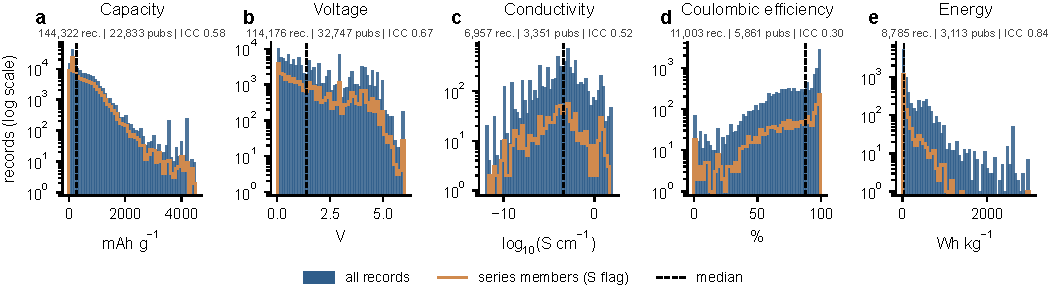
\includegraphics[width=\linewidth]{figures/fig_target_distributions.pdf}
    \caption{\textbf{Distributions of the five targets after cleaning} (log-scaled counts, 50 bins). Filled bars show all records and the orange outline the records flagged as within-paper series members (S); the dashed line marks the median. Above each panel: records, publications and the between-publication share of variance, ICC(1). Conductivity is shown as $\log_{10}(\sigma/\mathrm{S\,cm^{-1}})$.}
    \label{fig:dist}
\end{figure}

Table~\ref{tab:split} and Figure~\ref{fig:split}a report the main model ($t_2$) for each target under the three protocols. For capacity, $R^2$ fell from 0.529 $\pm$ 0.009 under record-level splitting to 0.477 $\pm$ 0.015 under DOI-grouped splitting and 0.398 $\pm$ 0.021 under temporal splitting, and MAE rose from 195 $\pm$ 1 to 213 $\pm$ 4~mAh~g$^{-1}$. The other targets behave in the same way. DOI grouping lowered $R^2$ from 0.499 $\pm$ 0.003 to 0.466 $\pm$ 0.010 for voltage, from 0.253 $\pm$ 0.016 to 0.213 $\pm$ 0.015 for conductivity, from 0.091 $\pm$ 0.017 to 0.068 $\pm$ 0.007 for Coulombic efficiency and from 0.538 $\pm$ 0.044 to 0.463 $\pm$ 0.080 for energy. The gaps (0.02--0.08) are small given the strong between-publication structure. A large between-publication share is necessary but not sufficient for a record-level advantage: the model must also be able to recognise the publication from its features, and Section~\ref{sec:channels} shows directly that the descriptors here carry little publication identity. With five targets we do not read anything into the ordering of the gaps by ICC(1). Every model beats the constant-mean baseline under every protocol, but Coulombic efficiency only marginally ($R^2 \le 0.1$). The per-specifier median baseline was worse than the constant mean for every target (DOI-grouped capacity RMSE 522 against 488 $\pm$ 4~mAh~g$^{-1}$), so the specifier alone explains little of the variance; its value lies in interaction with the composition.

Under record-level splitting, 90.0\% of test records came from publications that also contributed training records. Under DOI-grouped splitting this share is zero, but 71.2\% of test records had a compound name that occurs in training, compared with 92.0\% under random splitting and 66.1\% under temporal splitting. The DOI-grouped result is therefore an estimate of performance on new papers about largely familiar materials, and the temporal result is closer to performance on new materials. Temporal splitting was the strictest of the three publication-level protocols for every target: relative to DOI grouping, capacity lost a further 0.078 in $R^2$, and the shortfall was largest for energy. Later publications report more materials that are absent from earlier ones (66.1\% of temporal test records had a known name, against 71.2\% under DOI grouping), so the temporal estimate is closer to prospective use. Holding out whole compositions was stricter than DOI grouping for every target and stricter than the temporal split for voltage, conductivity and energy, with a large spread between splits: capacity reached 0.428 $\pm$ 0.081, voltage 0.387 $\pm$ 0.048 and conductivity 0.050 $\pm$ 0.054 (Table~\ref{tab:channels}). The disjoint five-fold grouped check reproduced the repeated-holdout DOI estimates (capacity 0.471 $\pm$ 0.013).

\begin{table}[htbp]
    \centering\small
    \caption{\textbf{Main model ($t_2$) under record-level random, DOI-grouped and temporal evaluation.} Mean $\pm$ sample standard deviation over splits (5, 5 and 3). $N$ is the mean number of test records per split. Units of MAE and RMSE: mAh~g$^{-1}$ (capacity), V (voltage), decades of S~cm$^{-1}$ (conductivity), percentage points (Coulombic efficiency), Wh~kg$^{-1}$ (energy). The last column is the constant-mean baseline RMSE on the DOI-grouped splits.}
    \label{tab:split}
    \begin{adjustbox}{max width=\textwidth}
    \begin{tabular}{@{}llrcccc@{}}
        \toprule
        Target & Protocol & $N$ & $R^2$ & MAE & RMSE & Baseline RMSE \\
        \midrule
        Capacity & Random   & 28,865 & 0.529 $\pm$ 0.009 & 195 $\pm$ 1 & 335 $\pm$ 3 & \\
        & DOI      & 28,486 & 0.477 $\pm$ 0.015 & 213 $\pm$ 4 & 353 $\pm$ 5 & 488 $\pm$ 4 \\
        & Temporal & 25,049 & 0.398 $\pm$ 0.021 & 244 $\pm$ 14 & 383 $\pm$ 8 & \\
        \midrule
        Voltage  & Random   & 22,836 & 0.499 $\pm$ 0.003 & 0.795 $\pm$ 0.003 & 1.062 $\pm$ 0.004 & \\
        & DOI      & 22,634 & 0.466 $\pm$ 0.010 & 0.834 $\pm$ 0.008 & 1.10 $\pm$ 0.01 & 1.50 $\pm$ 0.01 \\
        & Temporal & 18,686 & 0.396 $\pm$ 0.010 & 0.847 $\pm$ 0.020 & 1.10 $\pm$ 0.02 & \\
        \midrule
        Conductivity ($\log_{10}$) & Random & 1,392 & 0.253 $\pm$ 0.016 & 1.69 $\pm$ 0.03 & 2.31 $\pm$ 0.05 & \\
        & DOI      & 1,413 & 0.213 $\pm$ 0.015 & 1.73 $\pm$ 0.10 & 2.32 $\pm$ 0.11 & 2.61 $\pm$ 0.12 \\
        & Temporal & 1,100 & 0.197 $\pm$ 0.020 & 1.71 $\pm$ 0.19 & 2.33 $\pm$ 0.21 & \\
        \midrule
        Coulombic eff. & Random & 2,201 & 0.091 $\pm$ 0.017 & 15.4 $\pm$ 0.2 & 19.9 $\pm$ 0.4 & \\
        & DOI      & 2,179 & 0.068 $\pm$ 0.007 & 15.7 $\pm$ 0.4 & 20.0 $\pm$ 0.8 & 20.8 $\pm$ 0.8 \\
        & Temporal & 1,672 & 0.043 $\pm$ 0.009 & 15.9 $\pm$ 0.4 & 20.4 $\pm$ 0.3 & \\
        \midrule
        Energy   & Random   & 1,757 & 0.538 $\pm$ 0.044 & 132 $\pm$ 11 & 262 $\pm$ 27 & \\
        & DOI      & 1,775 & 0.463 $\pm$ 0.080 & 149 $\pm$ 6 & 281 $\pm$ 23 & 384 $\pm$ 11 \\
        & Temporal & 1,406 & 0.342 $\pm$ 0.058 & 137 $\pm$ 13 & 266 $\pm$ 18 & \\
        \bottomrule
    \end{tabular}
    \end{adjustbox}
\end{table}

\begin{figure}[htbp]
    \centering
    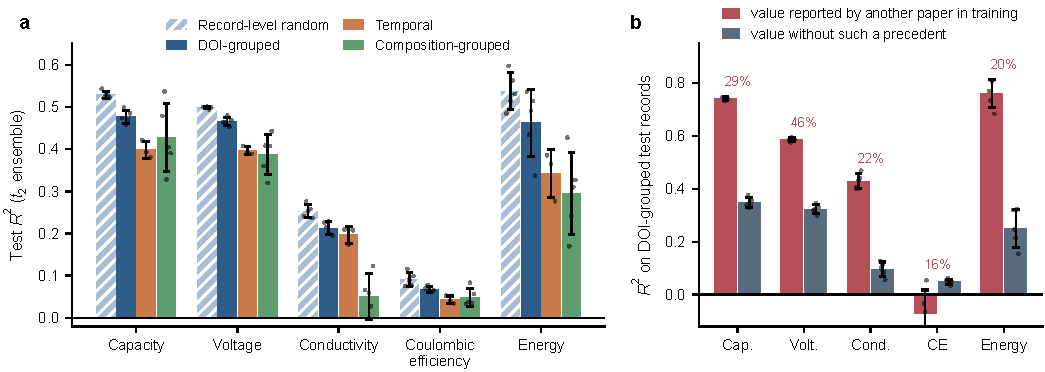
\includegraphics[width=\linewidth]{figures/fig_split_by_target.pdf}
    \caption{\textbf{Effect of the split protocol and of values recurring across publications.} (a) Test $R^2$ of the $t_2$ ensemble under record-level random (hatched), DOI-grouped, temporal and composition-grouped evaluation. (b) $R^2$ on DOI-grouped test records whose (normalised name, value) pair also occurs in a training record of another publication (red) and on the remaining records (grey); percentages give the share of test records with such a precedent. $R^2$ is computed within each subset; the negative value for repeated Coulombic-efficiency records reflects a constant underestimate of values reported as 95--100\%. Bars and error bars are the mean and sample standard deviation over splits (5, 5, 3 and 5); dots are individual splits.}
    \label{fig:split}
\end{figure}

\subsection{Why the DOI-grouped gap is small: leakage channels}
\label{sec:channels}

The small gap could mean that records from one publication are nearly independent, but Table~\ref{tab:targets} shows the opposite. Under record-level splitting, predicting each test record by the mean of the training records from its own publication, with no information about the material, gives $R^2$ of 0.39 for capacity, 0.48 for voltage and 0.33 for energy, a large fraction of what the full model achieves (and nearly all of it for voltage). Publication identity is therefore a strong predictor. The model does not exploit it because its features cannot recover it: from the composition descriptors, the journal of a record is predicted with a micro-F1 of 0.14 when publications are shared between training and test but only 0.02 when they are not, the publication year barely improves on the training mean, and a model given only the predicted journal and year has $R^2 \approx 0$ under both splits (Section~\ref{sec:previous}). In databases whose records carry process settings, device architectures or characteristic patterns of missing fields, such combinations can be specific to a laboratory and let a record-level split recognise the source; the battery records carry almost none of them.

A second channel is not blocked by DOI grouping (Figure~\ref{fig:split}b). Under DOI-grouped splitting, 29.1\% of capacity test records, 46.0\% of voltage records and 22.4\% of conductivity records repeat a (compound name, value) pair that another publication reported in the training set (Table~\ref{tab:channels}). These records are predicted far better than the rest: capacity $R^2$ was 0.74 on repeated and 0.35 on non-repeated records, and voltage 0.59 against 0.32. The repeated share and its advantage are almost the same under record-level splitting (capacity 30.7\%, $R^2$ 0.74), which is why the two protocols give similar overall scores: both reward recall of values that recur across the literature. Conductivity and Coulombic efficiency are not usefully predictable from this database. For conductivity, most of the DOI-grouped score comes from recalled values: $R^2$ is 0.43 on repeated records and 0.10 on the rest. Coulombic efficiency is not predicted on either subset (-0.07 and 0.05); its repeated values are mostly round numbers at the top of the scale (about a third are exactly 100\%), which the model, predicting about 81\% for almost every record, underestimates by about 9 percentage points, so that $R^2$ on this subset is negative although its MAE is slightly lower than on the other records, and for both targets Gaussian-noise columns receive about a quarter of the SHAP attribution (Section~\ref{sec:shap}). Their low overall scores should therefore not be read as weaker versions of the capacity result; they show what remains when recall of repeated values is removed. Theoretical capacities, which are a deterministic function of composition, make up 4.4\% of DOI-grouped capacity test records; excluding them lowers capacity $R^2$ from 0.477 $\pm$ 0.015 to 0.451.

\textbf{Robustness of the repeated-value analysis.} Exact matching undercounts restatements that were rounded differently. Matching within 1\% of the value raises the repeated share to 45.3\% for capacity, 49.9\% for voltage and 25.1\% for energy, with the same contrast (capacity $R^2$ 0.68 on repeated and 0.30 on other records), and rounding to two significant figures gives similar shares (Supporting Information, Table~S8). Repeated pairs are not a product of review articles: repeated test records come from publications with a median of 8 capacity records, against 12 for the other records, and the R flag is rare in both groups (3.9\% versus 1.4\%). Publication dates do not separate quotation from re-measurement here: the test publication is later than every matching publication for 20.2\% of repeated capacity records and earlier for 22.3\%, which is the near-symmetry expected when publications are assigned to training and test at random, whatever the mechanism. Among repeated capacity records, 16.7\% are theoretical capacities by specifier or by value. A sample of 50 repeated pairs with both source records is provided in the repository for inspection.

\begin{table}[htbp]
    \centering\small
    \caption{\textbf{Leakage channels by target} ($t_2$ ensemble; mean over splits). Same-pub.: $R^2$ of the same-publication mean under record-level splitting. Repeated: share of DOI-grouped test records whose (name, value) pair occurs in a training record of another publication, with $R^2$ on repeated and non-repeated records. Comp.-grouped: $R^2$ under composition-grouped splitting.}
    \label{tab:channels}
    \begin{adjustbox}{max width=\textwidth}
    \begin{tabular}{@{}lccccc@{}}
        \toprule
        Target & Same-pub.\ $R^2$ & Repeated share (DOI) & $R^2$ repeated & $R^2$ non-repeated & Comp.-grouped $R^2$ \\
        \midrule
        Capacity       & 0.39 & 29.1\% & 0.74 & 0.35 & 0.428 $\pm$ 0.081 \\
        Voltage        & 0.48 & 46.0\% & 0.59 & 0.32 & 0.387 $\pm$ 0.048 \\
        Conductivity   & 0.09 & 22.4\% & 0.43 & 0.10 & 0.050 $\pm$ 0.054 \\
        Coulombic eff. & -0.05 & 15.7\% & -0.07 & 0.05 & 0.049 $\pm$ 0.021 \\
        Energy         & 0.33 & 20.0\% & 0.76 & 0.25 & 0.295 $\pm$ 0.096 \\
        \bottomrule
    \end{tabular}
    \end{adjustbox}
\end{table}

\subsection{Effect of the paper-level (title-keyword) features and controls}
\label{sec:tiers}

Table~\ref{tab:tiers} reports DOI-grouped $R^2$ for every tier and target. Adding elemental-property statistics to composition ($t_{\mathrm{comp}} \rightarrow t_1$) changed $R^2$ by +0.002 for capacity, and adding the name and measurement-context blocks ($t_1 \rightarrow t_2$) by +0.038. Elemental-property statistics add almost nothing to the element fractions, as expected for a block that is a function of composition. The name and measurement-context blocks add most for capacity, where the specifier separates theoretical from measured values and current density and cycle number carry the measurement conditions, and little for Coulombic efficiency..

\textbf{Noise control.} The 32 noise columns changed DOI-grouped $R^2$ by -0.016 to -0.002 across targets and received 5.5--25.5\% of the total SHAP attribution (Table~\ref{tab:shap}). The models do not benefit from noise, but for the weak conductivity and Coulombic-efficiency models the noise columns receive about a quarter of the attribution: when the signal is weak, TreeSHAP spreads attribution over whatever the trees split on, and the feature rankings for these two targets should not be interpreted.

\textbf{Paper-level title keywords.} Adding title keywords and the R flag ($t_3 - t_2$) changed $R^2$ by +0.045 under random splitting and by +0.046 (95\% CI +0.040 to +0.052) under DOI-grouped splitting for capacity (Supporting Information, Table~S5). Unlike the paper-level features that are usually suspected of identifying publications, the title keywords help almost as much under DOI grouping as under random splitting for capacity and voltage, somewhat less for energy and Coulombic efficiency, and not significantly for conductivity; the gain is largest for energy ($\Delta R^2$ +0.064 (95\% CI +0.047 to +0.081)). They therefore carry chemistry rather than identity: the formula of the active material does not say whether it was tested in a lithium-ion, sodium-ion, Li--S or Li--O$_2$ cell, and the title does. This is the largest gain of any feature block we tested. We keep the title keywords out of the main tier only as a conservative choice, because the information is constant within a publication and describes how a paper presents its system rather than the material; a model that includes them ($t_3$, Table~\ref{tab:tiers}) is equally legitimate when the cell chemistry is known, and reaches DOI-grouped $R^2$ of 0.523 $\pm$ 0.014 for capacity, 0.509 $\pm$ 0.004 for voltage and 0.526 $\pm$ 0.064 for energy.

\textbf{Identity admission.} Adding the compound name as a categorical variable ($t_{2,\mathrm{id}} - t_2$) changed DOI-grouped $R^2$ by +0.002 for capacity and by -0.006 to +0.010 across targets. Under DOI grouping the effect is within $\pm0.01$ for every target (positive only for energy, +0.010 (95\% CI +0.003 to +0.018)); under random splitting the name added slightly more (capacity +0.009), a mild identity effect that largely disappears when publications are separated. Because the composition block already nearly determines the material, the name adds little beyond it.

\begin{table}[htbp]
    \centering\small
    \caption{\textbf{DOI-grouped $R^2$ by feature tier} (mean $\pm$ sample standard deviation over five splits; same splits for all tiers).}
    \label{tab:tiers}
    \begin{adjustbox}{max width=\textwidth}
    \begin{tabular}{@{}lccccc@{}}
        \toprule
        Tier & Capacity & Voltage & Conductivity & Coulombic eff. & Energy \\
        \midrule
        $t_{\mathrm{comp}}$     & 0.437 $\pm$ 0.014 & 0.452 $\pm$ 0.010 & 0.199 $\pm$ 0.012 & 0.060 $\pm$ 0.010 & 0.442 $\pm$ 0.067 \\
        $t_1$                   & 0.439 $\pm$ 0.013 & 0.455 $\pm$ 0.010 & 0.202 $\pm$ 0.016 & 0.069 $\pm$ 0.006 & 0.440 $\pm$ 0.075 \\
        $t_2$ (main)            & 0.477 $\pm$ 0.015 & 0.466 $\pm$ 0.010 & 0.213 $\pm$ 0.015 & 0.068 $\pm$ 0.007 & 0.463 $\pm$ 0.080 \\
        $t_3$                   & 0.523 $\pm$ 0.014 & 0.509 $\pm$ 0.004 & 0.218 $\pm$ 0.015 & 0.084 $\pm$ 0.011 & 0.526 $\pm$ 0.064 \\
        $t_{2,\mathrm{id}}$     & 0.478 $\pm$ 0.014 & 0.466 $\pm$ 0.010 & 0.207 $\pm$ 0.007 & 0.063 $\pm$ 0.009 & 0.473 $\pm$ 0.075 \\
        $t_{2,\mathrm{noise}}$  & 0.475 $\pm$ 0.013 & 0.459 $\pm$ 0.010 & 0.196 $\pm$ 0.015 & 0.058 $\pm$ 0.005 & 0.457 $\pm$ 0.069 \\
        \bottomrule
    \end{tabular}
    \end{adjustbox}
\end{table}



\subsection{Prediction distribution and errors}
\label{sec:prediction_diagnostics}

\textbf{Predicted versus reported values.} Figure~\ref{fig:diag} pools the DOI-grouped test predictions of the five splits. For capacity, voltage and energy the predictions follow the reported values but are compressed towards the centre of the distribution, and the predicted distributions are narrower than the reported ones. For Coulombic efficiency the model predicts values near 80\% for almost every record and misses the large mass of reported values close to 100\%; for conductivity it captures the main mode but not the tails. These patterns match the low $R^2$ of the last two targets and the under-prediction of high values discussed below.

\begin{figure}[htbp]
    \centering
    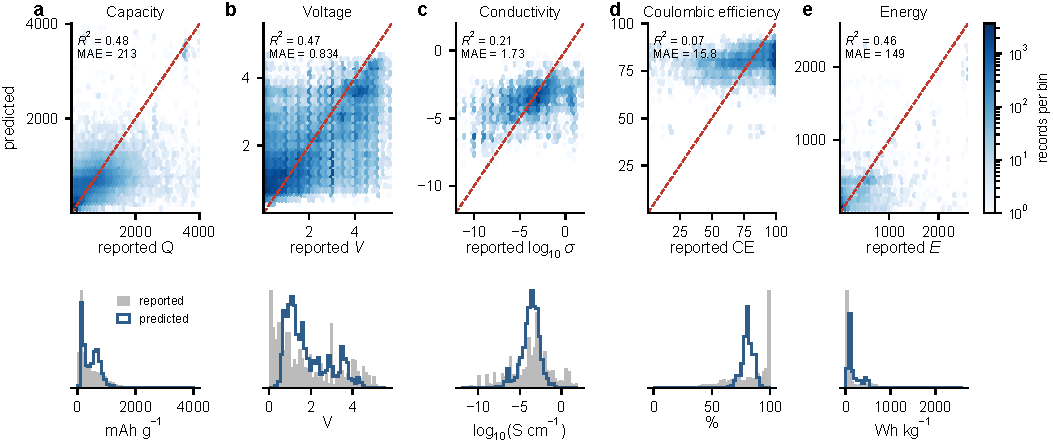
\includegraphics[width=\linewidth]{figures/fig_diagnostics.pdf}
    \caption{\textbf{Prediction diagnostics of the $t_2$ ensemble on DOI-grouped test records} (five splits pooled; a record can appear in more than one test set). Top: predicted versus reported values (log-scaled hexagonal bins; dashed line $y=x$), with $R^2$ and MAE of the pooled predictions. Bottom: distributions of reported (grey) and predicted (blue outline) values on the same axes.}
    \label{fig:diag}
\end{figure}

\textbf{Member spread and absolute error.} Figure~\ref{fig:unc} relates the spread of the ensemble members to the error. The Spearman correlation between member spread and absolute error was 0.39 for capacity under DOI-grouped evaluation and 0.35 under random evaluation (Supporting Information, Table~S6). The mean spread for DOI-grouped test records was 1.03 times that for record-level test records. Records in the top decile of spread had an MAE of 367, compared with 85.9 in the bottom decile. The spread is informative only for capacity and energy ($\rho \approx 0.35$); for voltage, conductivity and Coulombic efficiency $\rho \le 0.16$. It rises only slightly for publications not seen in training (ratio 1.03--1.17), much less than the error does. Four members that share data and hyperparameters are not a substitute for a calibrated interval, and we use the spread only to rank records for inspection.



\begin{figure}[htbp]
    \centering
    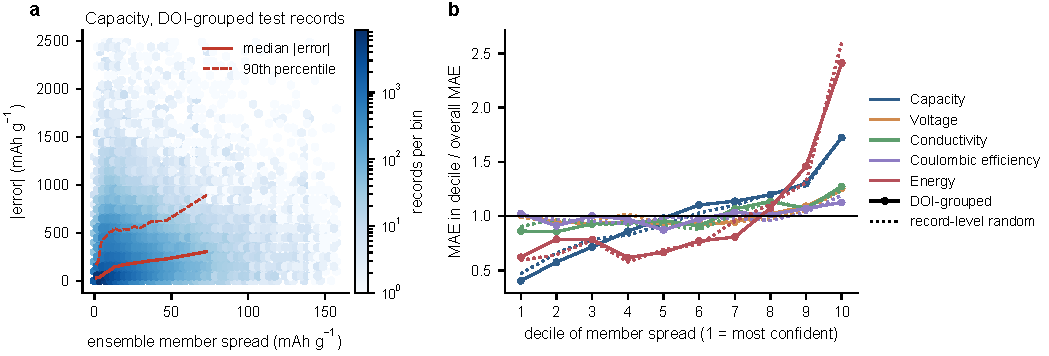
\includegraphics[width=\linewidth]{figures/fig_uncertainty.pdf}
    \caption{\textbf{Ensemble spread and error.} (a) Absolute error versus ensemble member spread for capacity on the DOI-grouped test records of all five splits (log-scaled hexagonal bins), with the median and 90th percentile of the absolute error in 20 quantile bins of spread. (b) MAE in each decile of member spread divided by the overall MAE, for each target under DOI-grouped (solid, markers) and record-level random (dotted) evaluation.}
    \label{fig:unc}
\end{figure}

\textbf{High-value errors.} Predictions regress towards the mean. Under DOI-grouped evaluation the decile of highest reported capacities (mean 1533~mAh~g$^{-1}$) was under-predicted by -645~mAh~g$^{-1}$ on average and the lowest decile (mean 53.9) over-predicted by 220; the same pattern holds for voltage (top decile 4.67~V, bias -1.40~V) and energy. Many of the extreme values are near the L-flag limits and include extraction errors, so part of this bias is the correct response of a regularised model to label noise; the model should not be used to rank candidate materials by extreme predicted capacity..

\textbf{Within-paper series.}\label{sec:series} Removing S-flagged records reduced the capacity set to 62,717 records. The record-level minus DOI-grouped gap in $R^2$ was 0.052 with series records and 0.024 without them (Table~\ref{tab:series}). Series members are therefore the main channel through which record-level splitting rewards within-publication similarity: without them the record-level advantage shrinks for every target except Coulombic efficiency, and both protocols score higher, because series members are the records whose values depend most on measurement conditions (current density, cycle number) that the features describe only partly. Removing S also changes the population, so the absolute values with and without S are not a like-for-like comparison of model quality.

\begin{table}[htbp]
    \centering\small
    \caption{\textbf{Sensitivity to within-paper series.} $R^2$ of the $t_2$ ensemble with all records and with S-flagged records removed.}
    \label{tab:series}
    \begin{adjustbox}{max width=\textwidth}
    \begin{tabular}{@{}lcccc@{}}
        \toprule
        & \multicolumn{2}{c}{All records} & \multicolumn{2}{c}{Without S} \\
        \cmidrule(lr){2-3}\cmidrule(l){4-5}
        Target & Random & DOI & Random & DOI \\
        \midrule
        Capacity       & 0.529 $\pm$ 0.009 & 0.477 $\pm$ 0.015 & 0.551 $\pm$ 0.017 & 0.527 $\pm$ 0.004 \\
        Voltage        & 0.499 $\pm$ 0.003 & 0.466 $\pm$ 0.010 & 0.497 $\pm$ 0.004 & 0.480 $\pm$ 0.009 \\
        Conductivity   & 0.253 $\pm$ 0.016 & 0.213 $\pm$ 0.015 & 0.247 $\pm$ 0.031 & 0.222 $\pm$ 0.012 \\
        Coulombic eff. & 0.091 $\pm$ 0.017 & 0.068 $\pm$ 0.007 & 0.088 $\pm$ 0.008 & 0.064 $\pm$ 0.007 \\
        Energy         & 0.538 $\pm$ 0.044 & 0.463 $\pm$ 0.080 & 0.514 $\pm$ 0.058 & 0.500 $\pm$ 0.074 \\
        \bottomrule
    \end{tabular}
    \end{adjustbox}
\end{table}

\textbf{Data quality of the extracted records.} Four consequences of the extraction errors described in Section~\ref{sec:quality} follow. First, with roughly one record in five wrong in at least one field, the achievable $R^2$ is bounded well below one even for a perfect model, and errors in the value or the property assignment act as label noise that no feature can explain. Second, F1 and F2 errors corrupt the composition features themselves; the raw file contains, for example, a record named ``Carbon'' whose parsed composition is C$_{12}$H$_{22}$O$_{11}$ (sucrose, presumably the carbon source in that paper). Third, because the evaluation sample was augmented for rare properties, it is not a simple random sample, and the precision values should be taken as approximate. Fourth, the Correctness sample is too small to estimate model error separately for correct and incorrect records with any precision; we report descriptively that the DOI-grouped absolute error of the 353 labelled records that fell in test partitions was 148~mAh~g$^{-1}$ ($n=138$, capacity) for records marked correct and 232~mAh~g$^{-1}$ ($n=26$) for those marked incorrect. Our physical-range filter removes only the grossest errors; values that are wrong but plausible remain.

\subsection{Interpretation of model predictions}
\label{sec:shap}

Table~\ref{tab:shap} and Figure~\ref{fig:shap} give the share of mean $|$SHAP$|$ by feature group for the $t_2$ ensembles under DOI-grouped evaluation (and for the noise columns in $t_{2,\mathrm{noise}}$). For capacity, measurement-context features accounted for 17.0\%, composition for 21.5\%, elemental properties for 57.6\% and name flags for 3.9\%. The highest-ranked individual feature was \texttt{mat\_ie1\_range} (76.5~mAh~g$^{-1}$). Elemental-property statistics carry the largest share for every target (50--70\%), composition fractions most of the remainder, and the name flags less than 5\%. Measurement context matters mainly for capacity (17.0\%), where the specifier and current density distinguish theoretical from measured and low-rate from high-rate values, and hardly at all for Coulombic efficiency. The leading individual features are chemically plausible: silicon fraction and ionisation-energy and group statistics for capacity, Mendeleev-number and electronegativity ranges and lithium fraction for voltage, and lithium content for energy, which is dominated by Li--S and Li--O$_2$ systems at the high end. For conductivity and Coulombic efficiency the noise control shows that rankings are unreliable (Section~\ref{sec:tiers}).

Attributions to composition and elemental-property features should be read with care. Elemental statistics are functions of composition and can act as a coordinate system for recognising familiar materials; a high attribution does not mean the model has learned a physical relationship between, for example, electronegativity and voltage.

\begin{table}[htbp]
    \centering\small
    \caption{\textbf{Share of mean $|$SHAP$|$ by feature group} ($t_2$ ensembles, DOI-grouped test records; mean over five splits; noise share from $t_{2,\mathrm{noise}}$).}
    \label{tab:shap}
    \begin{adjustbox}{max width=\textwidth}
    \begin{tabular}{@{}lccccc@{}}
        \toprule
        Group & Capacity & Voltage & Conductivity & Coulombic eff. & Energy \\
        \midrule
        Composition    & 21.5\% & 26.8\% & 38.8\% & 25.0\% & 42.6\% \\
        Material       & 57.6\% & 63.1\% & 53.4\% & 69.8\% & 50.3\% \\
        Material name  & 3.9\% & 2.8\% & 4.5\% & 4.9\% & 4.9\% \\
        Measurement    & 17.0\% & 7.4\% & 3.4\% & 0.3\% & 2.1\% \\
        \midrule
        Noise ($t_{2,\mathrm{noise}}$) & 5.5\% & 7.9\% & 22.9\% & 25.5\% & 11.6\% \\
        \bottomrule
    \end{tabular}
    \end{adjustbox}
\end{table}

\begin{figure}[htbp]
    \centering
    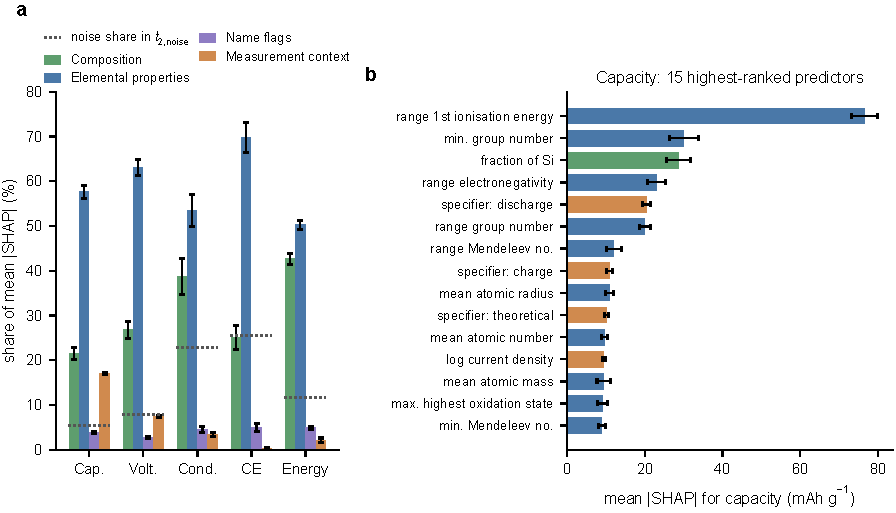
\includegraphics[width=\linewidth]{figures/fig_shap_groups_by_target.pdf}
    \caption{\textbf{Grouped SHAP attribution} ($t_2$ ensembles, DOI-grouped test records). (a) Share of the total mean $|$SHAP$|$ by feature group for each target; dotted lines give the share taken by the 32 Gaussian-noise columns in the $t_{2,\mathrm{noise}}$ control. (b) The 15 highest-ranked predictors for capacity, coloured by group as in (a). Bars are means and error bars sample standard deviations over the five splits.}
    \label{fig:shap}
\end{figure}

\subsection{Comparison with previous studies on the Huang--Cole database}
\label{sec:previous}

Screening the 167 works that cite the database in the Semantic Scholar index (November 2026) found two groups that train models on its records (Table~\ref{tab:previous}); most other citing works are reviews, extraction tools or databases for other properties. Zhuang and Barnard used its formulas to study composition encodings, first by clustering and classifying the encoded formulas \cite{zhuang2023mendeleev,zhuang2024classification,zhuang2025applications} and then by regression \cite{zhuang2024property}: the Mendeleev+ encoding with XGBoost, trained on 254,749 cleaned records with a random 85/15 split, gave test $R^2$ of 0.47--0.50 for capacity, voltage and energy and below 0.15 for Coulombic efficiency and conductivity, and nearly the same values when only one record per formula was kept. Jablonka used 33,701 unflagged capacity records as one of five case studies of bibliographic confounding, with 273 matminer descriptors \cite{ward2018matminer,ward2016magpie,meredig2014combinatorial} and default LightGBM \cite{ke2017lightgbm} evaluated by random 10-fold cross-validation, and recommended group and time splits as routine falsification tests \cite{jablonka2026clever}.

\begin{table}[htbp]
    \centering\small
    \caption{\textbf{Previous studies that model records of the Huang--Cole database, and this work.} Values are as reported by each study; tasks, record selection and evaluation differ, so rows are not directly comparable.}
    \label{tab:previous}
    \begin{adjustbox}{max width=\textwidth}
    \begin{tabular}{@{}p{2.6cm} p{2.6cm} p{3.0cm} p{2.4cm} p{2.6cm} p{2.2cm}@{}}
        \toprule
        Study & Task & Records & Features / model & Evaluation & Reported \\
        \midrule
        Zhuang \& Barnard \cite{zhuang2024classification} & cluster label (2 or 5 classes) & 265,481 cleaned formula instances & Mendeleev encodings; LR, DT, SVM & random stratified 85/15; 7-fold CV & accuracy 0.99--1.00 \\
        Zhuang \& Barnard \cite{zhuang2024property} & five properties (regression) & 254,749 cleaned records; one-per-formula variant & Mendeleev+ encoding; XGBoost (1,000-combination search) & random 85/15; 10-fold CV & $R^2$ capacity 0.473, voltage 0.489, energy 0.495, CE 0.142, cond.\ 0.056 \\
        Jablonka \cite{jablonka2026clever} & capacity; author, journal, year & 33,701 capacity records (merged release, no warning flag) & 273 matminer descriptors; LightGBM (default) & random 10-fold CV & metadata predictable; metadata-only model $\approx$ mean \\
        \midrule
        This work & five properties & 285,243 records, 42,840 publications & composition, elemental, name and measurement features; CatBoost--XGBoost & random / DOI-grouped / temporal, 5 repeats & capacity $R^2$ 0.529 $\pm$ 0.009 / 0.477 $\pm$ 0.015 / 0.398 $\pm$ 0.021 \\
        \bottomrule
    \end{tabular}
    \end{adjustbox}
\end{table}

\textbf{Adapted pipelines on common partitions.} We ran the public code of Jablonka unchanged (composition parsing, descriptors, preprocessing and model) on our split-1 partitions; as in that code, records with any non-computable descriptor are dropped, which keeps 92\%--96\% of the test records, and the ensemble is scored on the same subset. The Zhuang--Barnard regression notebook is part of the supporting information of their article, so we re-implemented the workflow from their Methods with a smaller hyperparameter search (25 configurations, 3-fold cross-validation on at most 20,000 records, instead of 1,000 with 10-fold). Table~\ref{tab:adapted} gives both pipelines for every target. The comparison asks whether the protocol effect is specific to our workflow, not which model is best, and the ensemble is not uniformly better (for DOI-grouped conductivity the adapted Jablonka pipeline scores higher). We use one partition because each adapted pipeline needs its own featurisation and, for Zhuang--Barnard, its own hyperparameter search; differences smaller than the split-to-split standard deviations in Table~\ref{tab:split} (up to 0.08, for energy) are not interpreted. On the records released by Zhuang and Barnard, the re-implementation reproduced their random-split $R^2$ for capacity (0.471 versus 0.473) and voltage to within 0.01, and a DOI-grouped split lowered capacity $R^2$ to 0.411 (Supporting Information, Table~S7): the same moderate, target-dependent effect that we find with our own records, features and model.

\begin{table}[htbp]
    \centering\small
    \caption{\textbf{Adapted pipelines of Jablonka \cite{jablonka2026clever} and Zhuang and Barnard \cite{zhuang2024property} and the CatBoost--XGBoost ensemble on common partitions} (split~1; each adapted pipeline is paired with the ensemble scored on exactly the test records that pipeline can featurise; single-partition values without standard deviations). Cells give $R^2$ / MAE; MAE units as in Table~\ref{tab:split}.}
    \label{tab:adapted}
    \begin{adjustbox}{max width=\textwidth}
    \begin{tabular}{@{}llccccc@{}}
        \toprule
        Split & Model & Capacity & Voltage & Conductivity & Coulombic eff. & Energy \\
        \midrule
        Random & Jablonka, adapted & 0.467 / 219 & 0.454 / 0.842 & 0.223 / 1.72 & 0.069 / 15.2 & 0.486 / 133 \\
        & \quad ensemble, same records & 0.543 / 194 & 0.492 / 0.798 & 0.240 / 1.70 & 0.078 / 15.2 & 0.486 / 143 \\
        & Zhuang--Barnard, adapted & 0.482 / 213 & 0.470 / 0.826 & 0.198 / 1.76 & 0.074 / 15.1 & 0.479 / 129 \\
        & \quad ensemble, same records & 0.542 / 194 & 0.492 / 0.797 & 0.240 / 1.70 & 0.078 / 15.2 & 0.486 / 143 \\
        \midrule
        DOI    & Jablonka, adapted & 0.429 / 225 & 0.430 / 0.869 & 0.240 / 1.77 & 0.035 / 15.0 & 0.543 / 133 \\
        & \quad ensemble, same records & 0.482 / 212 & 0.458 / 0.840 & 0.225 / 1.82 & 0.069 / 15.1 & 0.554 / 144 \\
        & Zhuang--Barnard, adapted & 0.442 / 221 & 0.445 / 0.850 & 0.214 / 1.81 & 0.029 / 15.0 & 0.512 / 135 \\
        & \quad ensemble, same records & 0.481 / 212 & 0.458 / 0.840 & 0.225 / 1.82 & 0.069 / 15.1 & 0.554 / 144 \\
        \bottomrule
    \end{tabular}
    \end{adjustbox}
\end{table}

\textbf{Bibliographic fingerprints.} Repeating Jablonka's metadata test with the journal and year in the database (author lists are not released), the descriptors predicted the journal noticeably better than chance only when publications were shared between training and test (capacity micro-F1 0.14 versus 0.02), and a model given only the predicted journal and year reached a capacity $R^2$ of 0.002 (random) and -0.001 (DOI-grouped), with the same result for every target (Supporting Information, Table~S1). In this database, descriptor-based fingerprints are weak and mostly reflect shared publications.

\textbf{Implications for evaluating models on text-mined data.} Clustered targets alone did not produce a large record-level advantage: a model can exploit only the publication identity that its inputs encode, so the random-versus-grouped comparison has to be run for each feature set rather than inferred from the between-publication variance. DOI grouping, in turn, cannot separate values that are restated across publications, and with an extraction precision of about 80\% such repetition can also propagate extraction errors. Composition-grouped and temporal splits, and the repeated/non-repeated breakdown, are needed to estimate performance on values without a precedent in the literature, which is the case that matters for discovery.

\subsection{Limitations}
\label{sec:limitations}

DOI-grouped evaluation tests performance on publications excluded from training; it does not guarantee independence of laboratories or research groups, and author information is not part of the release. Our repeated-value analysis matches on the normalised compound name, so it misses restatements under a different name, and the tolerance-based matches show that exact matching undercounts recurrence; neither publication dates nor rule-based classes distinguish quotation from independent re-measurement. Composition grouping uses rounded atomic fractions of the parsed formula and therefore treats composites with the same overall composition as one material. The targets mix quantities that a materials scientist would keep apart (theoretical and measured capacity, average and cut-off voltage, ionic and electronic conductivity), and the specifier flags only partly separate them. Material descriptors are computed from the parsed formula of the active material and ignore binders, conductive additives, electrolytes and counter electrodes \cite{kauwe2019battery}. The database ends with papers published in 2019, so the temporal split cannot test generalisation to recent chemistries. We use this release deliberately: the questions are methodological, and it is the database on which the previous models were trained and reported. The adapted pipelines keep the published featurisation and learner but are evaluated on our records and partitions, so they test the workflows on a common task and do not reproduce the published scores. Finally, the extraction errors discussed in Section~\ref{sec:quality} are not removed by any of our filters.

% ---------------- CONCLUSION ----------------
\section{Conclusions}
\label{sec:conclusion}

We trained CatBoost--XGBoost ensembles on the Huang--Cole auto-generated battery database for five properties and evaluated identical models under record-level, DOI-grouped, temporal and composition-grouped splits. Records are strongly clustered by publication, yet DOI grouping lowered $R^2$ by only 0.02--0.08 (capacity 0.529 $\pm$ 0.009 to 0.477 $\pm$ 0.015), because composition descriptors carry little recoverable publication identity. A larger effect comes from values that recur across publications: 16--46\% of DOI-grouped test records have such a precedent and are predicted much better than the rest, and on values without one capacity $R^2$ falls to 0.35 and conductivity and Coulombic efficiency are not usefully predicted (0.10 and 0.05). Temporal and composition-grouped splits lower performance further. Title keywords, which describe the cell chemistry, improve predictions under both split types, the raw compound name changes DOI-grouped $R^2$ by at most 0.01, Gaussian-noise columns receive 5.5--25.5\% of the attribution and do not improve any target, and removing within-paper series narrows the record-level advantage further.

Three recommendations follow for models trained on text-mined materials data. First, report publication-grouped results, but do not treat them as a test of generalisation to new materials: add composition-grouped or temporal splits and report performance separately for values with and without a precedent in the training literature. Second, check whether the features can identify publications, for example with the bibliographic-fingerprint test, before interpreting a small or large random-versus-grouped gap. Third, audit the database's own flags before use, because in this database one flag encodes publication identity and another is a function of the target. Future work should add the experimental context that the database lacks, separate theoretical from measured values at extraction time, and test whether newer extraction pipelines \cite{huang2022batterybert,dagdelen2024structured} change these conclusions.

\section{Data and Software Availability}
The Huang--Cole battery materials database analysed in this study is publicly available from figshare \cite{huang2020figshare} at \url{https://doi.org/10.6084/m9.figshare.11888115}. The code for data preparation, model training, evaluation and the adapted comparison pipelines, the frozen element list, the split fingerprints and all result tables are archived on Zenodo \cite{patel2026batteryprediction} (version v1.0.0) at \url{https://doi.org/10.5281/zenodo.24500203} and developed at \url{https://github.com/sunraj-patel/battery-prediction}. All software used is open source (Python with CatBoost, XGBoost, scikit-learn, SHAP, pymatgen, matminer and LightGBM); package requirements are listed in the archived repository. The adapted pipelines reuse code from \url{https://github.com/lamalab-org/clever-materials-hans} (MIT licence) and data files from \url{https://github.com/ZoraZhuang/battery_datasets} (GPL-3.0).

\begin{suppinfo}
Bibliographic-fingerprint test for all targets; columns excluded from the predictors with reasons; model configuration; split-protocol partition sizes; paper-level and identity controls under both split types; ensemble-spread statistics; re-run of the Zhuang--Barnard workflow on its own records; diagnostics of repeated (name, value) pairs (Tables S1--S8) (PDF)
\end{suppinfo}

\section*{Author Information}
\subsection*{Corresponding Author}
Sunraj Patel -- Department of Materials Science and Engineering, Indian Institute of Technology Kanpur, Kanpur 208016, India; Email: sunrajpatelcph@gmail.com
\subsection*{Author Contributions}
S.P.: conceptualisation, data curation, formal analysis, investigation, methodology, software, validation, visualisation, writing -- original draft, and writing -- review and editing.
\subsection*{Notes}
The author declares no competing financial interest.

\begin{acknowledgement}
This research did not receive any specific grant from funding agencies in the public, commercial or not-for-profit sectors. Computations were performed in part on PARAM Sanganak, provided under the National Supercomputing Mission (NSM), Government of India. The author thanks Shu Huang and Jacqueline M.\ Cole for releasing the battery database, and Kevin Maik Jablonka and Zixin Zhuang and Amanda S.\ Barnard for making their code and data public. During the preparation of this work, the author used Claude and Gemini to audit the code, clean up the final pipeline, format the manuscript, and improve its language. The author reviewed and edited the resulting content and takes full responsibility for the content of the published article.
\end{acknowledgement}

\bibliography{references_battery}

\end{document}
